\section{Motivation}
\begin{frame}{Differential Cryptanalysis}
    \begin{block}{SPN Cipher}
        \vspace{0.5em}
        \centering
        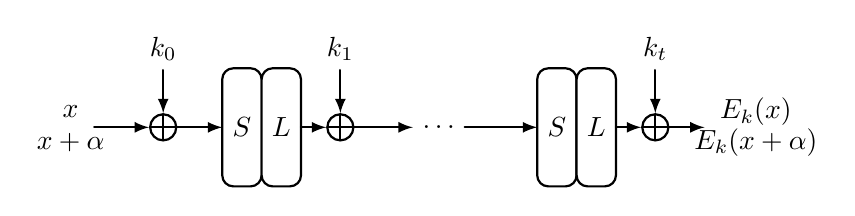
\begin{tikzpicture}[line cap=round]
            \tikzset{tikzxor/.style={draw,thick,circle,append after command={%
                    [shorten >=\pgflinewidth, shorten <=\pgflinewidth,]
                    (\tikzlastnode.north) edge[thick] (\tikzlastnode.south)
                    (\tikzlastnode.east) edge[thick] (\tikzlastnode.west)
                    }
                }
            }

            \node[tikzxor] (v1) at (-1.75,-4.25) {};
            \node[tikzxor] (v2) at (0.5,-4.25) {};
            \node[tikzxor] (v3) at (4.5,-4.25) {};

            \draw[thick, rounded corners, fill=white] (-1,-3.5) rectangle (-0.5,-5);
            \draw[thick, rounded corners, fill=white]  (-0.5,-3.5) rectangle (0,-5);
            \node at (-0.75,-4.25) {$S$};
            \node at (-0.25,-4.25) {$L$};

            \node (dots) at (1.75,-4.25) {$\dots$};
            \draw[thick, rounded corners, fill=white] (3,-3.5) rectangle (3.5,-5);
            \draw[thick, rounded corners, fill=white] (3.5,-3.5) rectangle (4,-5);
            \node at (3.25,-4.25) {$S$};
            \node at (3.75,-4.25) {$L$};

            \node (k0) at (-1.75,-3.25) {$k_0$};
            \draw [thick,-latex](k0) -- (v1);

            \node (k1) at (0.5,-3.25) {$k_1$};
            \draw [thick,-latex](k1) -- (v2);

            \node (kt) at (4.5,-3.25) {$k_t$};
            \draw [thick,-latex](kt) -- (v3);

            \node (x) at (-2.75,-4.25) {};
            \node [xshift=-5pt,yshift=2pt] at (x.north) {$x$};
            \node [xshift=-5pt,yshift=-2pt] at (x.south) {$x+\alpha$};
            \draw [thick,-latex](x) -- (v1);

            \node (Ekx) at (5.25,-4.25) {};
            \node [xshift=15pt,yshift=2pt] at (Ekx.north) {$E_k(x)$};
            \node [xshift=15pt,yshift=-2pt] at (Ekx.south) {$E_k(x+\alpha)$};
            \draw [thick,-latex](v3) -- (Ekx);

            \draw [thick,-latex](v1) -- (-1,-4.25);
            \draw [thick,-latex](0,-4.25) -- (v2);
            \draw [thick,-latex](v2) -- (dots);
            \draw [thick,-latex](dots) -- (3,-4.25);
            \draw [thick,-latex](4,-4.25) -- (v3);
        \end{tikzpicture}
        \vspace{0.5em}
    \end{block}
    \begin{block}{Definition~\cite{FSE:Knudsen94,FSE:BloLeaNyb14}}
        Let $F : \F_2^n \to \F_2^n$.
        A \emph{truncated differential} of probability one is a pair of affine subspaces $\coset{U}{s}$ and $\coset{V}{t}$ of $\F_2^n$, \st/
        \begin{equation*}
            \forall u \in U : \forall x \in \F_2^n : F(x) + F(x + u + s) \in \coset{V}{t}
        \end{equation*}
    \end{block}
\end{frame}

\begin{frame}{Structural Attacks}{Subspace Trail Cryptanalysis}
    \begin{block}{Main Idea}
        \centering
        \vspace{0.25em}
        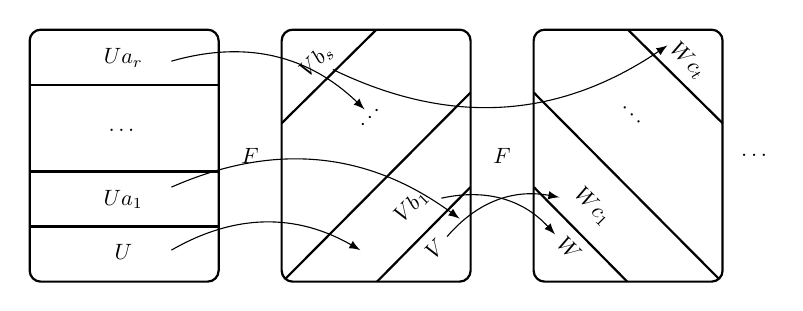
\begin{tikzpicture}[scale=0.8]
            \tikzstyle{every node}=[transform shape];

            \node (left2-space) [draw,rectangle,thick,rounded corners,minimum width=3cm,minimum height=4cm,fill=white] at (1,0) {};
            \draw[thick] (left2-space.west)+(0,1.125cm) -- node[above, yshift=1.5mm] {$\coset{U}{a_r}$} +(3cm,1.125cm);
            \draw[thick] (left2-space.west)+(0,-0.25cm) -- node[above, yshift=5mm] {\dots} +(3cm,-0.25cm);
            \draw[thick] (left2-space.west)+(0,-1.125cm) -- node[above, yshift=1.5mm] {$\coset{U}{a_1}$}
                                                            node[below, yshift=-1.5mm] {$U$} +(3cm,-1.125cm);

            \node (middle-space) [draw,rectangle,thick,rounded corners,minimum width=3cm,minimum height=4cm,fill=white] at (5,0) {};
            \draw[thick] (middle-space.north)+(0pt,-0.5pt) -- node[above, yshift=0.5mm, rotate=45] (vbs) {$\coset{V}{b_s}$} +(-1.5cm,-1.5cm);
            \draw[thick] (middle-space.east)+(-0.5pt,1cm) -- node[above, yshift=10mm, rotate=45] (middle-dots) {\dots} +(-3cm+1.25pt,-2cm+1.25pt);
            \draw[thick] (middle-space.east)+(-0.5pt,-5mm) -- node[above, yshift=2.5mm, rotate=45] (vb1) {$\coset{V}{b_1}$}
                                                        node[below, yshift=-0.5mm, rotate=45] (v) {$V$} +(-1.5cm,-2cm);

            \draw[-latex] (1.75,-0.5) to [bend left] (6.325,-1.0);
            \draw[-latex] (1.75,-1.5) to [bend left] (4.75,-1.5);
            \draw[-latex] (1.75,+1.5) to [bend left] (middle-dots);

            \node (left-f) at (3,0) {$F$};

            \visible<2->{%
            \node (right-space) [draw,rectangle,thick,rounded corners,minimum width=3cm,minimum height=4cm,fill=white] at (9,0) {};
            \draw[thick] (right-space.north)+(0pt,-0.5pt) -- node[above, yshift=0.5mm, rotate=-45] (wct) {$\coset{W}{c_t}$} +(+1.5cm,-1.5cm);
            \draw[thick] (right-space.west)+(0.5pt,1cm) -- node[above, yshift=10mm, rotate=-45] (right-dots) {\dots} +(3cm-1.25pt,-2cm+1.25pt);
            \draw[thick] (right-space.west)+(0.5pt,-5mm) -- node[above, yshift=2.5mm, rotate=-45] (wc1) {$\coset{W}{c_1}$}
                                                        node[below, yshift=-0.5mm, rotate=-45] (w) {$W$} +(+1.5cm,-2cm);

            \node (middle-f) at (7,0) {$F$};
            \node (right-f) at (11,0) {$\ldots$};

            \draw[-latex] (vb1) to [bend left] (w);
            \draw[-latex] (v) to [bend left] (wc1);
            \draw[-latex] (vbs) to [bend right] (9.625,+1.75);
            }
        \end{tikzpicture}
    \end{block}
    \visible<3->{%
    \begin{block}{Subspace Trail Cryptanalysis~\cite{ToSC:GraRecRon16} (Last Year's FSE)}
        \vspace{0.25em}
        Let $(U_0, \ldots, U_r)$ be subspaces of $\F_2^n$, and $F : \F_2^n \to \F_2^n$.
        We write
        \begin{equation*}
            U_0 \through{F} \cdots \through{F} U_r \Leftrightarrow 0 \leq i < r : \forall a \in U_i^\perp : \exists b \in U_{i+1}^\perp : F(\coset{U_i}{a}) \subseteq \coset{U_{i+1}}{b}
        \end{equation*}
    \end{block}
    }
\end{frame}

\begin{frame}{Outline}{}
    \begin{block}{Outline}
        \vspace{0.5em}
        \tableofcontents[sectionstyle=shaded/show]
    \end{block}
\end{frame}

\section{Link to Truncated Differentials}
%\begin{frame}{Preliminaries, Notations}
%    \begin{block}{Subspace Complement}
%        If $U$ is a subspace of $\F_2^n$, we denote by $U^\perp$ it's \emph{complement}:
%        \vspace{-0.5em}
%        \begin{equation*}
%            U^\perp \coloneqq \set{u \in \F_2^n \given \forall x \in U: \angles{x, u} = 0}
%            \vspace*{-0.5em}
%        \end{equation*}
%    \end{block}
%\end{frame}

\begin{frame}{Intuition}{The Image of the Derivative is in the Subspace}
    \begin{lemma}
        \vspace{0.5em}
        Let $U \through{F} V$ be a subspace trail.
        Then for all $x$: $F(x) + F(x + u) \in V$.
    \end{lemma}
    \begin{block}{Proof}
        \centering
        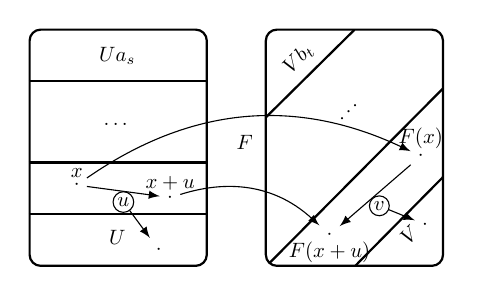
\begin{tikzpicture}[scale=0.75]
            \tikzstyle{every node}=[transform shape];

            \node (left2-space) [draw,rectangle,thick,rounded corners,minimum width=3cm,minimum height=4cm,fill=white] at (1,0) {};
            \draw[thick] (left2-space.west)+(0,1.125cm) -- node[above, yshift=1.5mm] {$\coset{U}{a_s}$} +(3cm,1.125cm);
            \draw[thick] (left2-space.west)+(0,-0.25cm) -- node[above, yshift=5mm] {\dots} +(3cm,-0.25cm);
            \draw[thick] (left2-space.west)+(0,-1.125cm) -- node[below, yshift=-1.5mm] {$U$} +(3cm,-1.125cm);

            \node (right2-space) [draw,rectangle,thick,rounded corners,minimum width=3cm,minimum height=4cm,fill=white] at (5,0) {};
            \draw[thick] (right2-space.north)+(0pt,-0.5pt) -- node[above, yshift=0.5mm, rotate=45] {$\coset{V}{b_t}$} +(-1.5cm,-1.5cm);
            \draw[thick] (right2-space.east)+(-0.5pt,1cm) -- node[above, yshift=10mm, rotate=45] {\dots} +(-3cm+1.25pt,-2cm+1.25pt);
            \draw[thick] (right2-space.east)+(-0.5pt,-5mm) -- node[below, yshift=-0.5mm, rotate=45] {$V$} +(-1.5cm,-2cm);

            \node[xshift=-20pt, yshift=-18pt] (x1) at (left2-space) {$\cdot$};
            \node[above] (x1-label) at (x1) {$x$};

            \node[xshift=32pt, yshift=-4pt] (y1) at (right2-space) {$\cdot$};
            \node[above] (y1-label) at (y1) {$F(x)$};

            \draw[-latex] (x1) to [bend left] node[below,yshift=-5pt] {$F$} (y1);

            \visible<2->{%
                \node[xshift=25pt, yshift=-24pt] (x2) at (left2-space) {$\cdot$};
                \node[above] (x2-label) at (x2) {$x+u$};

                \node[xshift=-12pt, yshift=-42pt] (y2) at (right2-space) {$\cdot$};
                \node[below] (y2-label) at (y2) {$F(x+u)$};

                \draw[-latex] (x1) -- node[below,draw,fill=white,inner sep=1pt,circle] (u-label) {$u$} (x2);
                \node[xshift=17pt, yshift=-23pt] at (u-label) (u) {$\cdot$};

                \draw[-latex] (u-label) -- (u);

                \draw[-latex] (x2) to [bend left] (y2);
            }

            \visible<3->{%
                \draw[-latex] (y1) -- node[below,xshift=2pt,draw,fill=white,inner sep=1pt,circle] (v-label) {$v$} (y2);
                \node[xshift=22pt, yshift=-9pt] at (v-label) (v) {$\cdot$};

                \draw[-latex] (v-label) -- (v);
            }

        \end{tikzpicture}
    \end{block}
\end{frame}

\begin{frame}{Link to Truncated Differentials}{Direct consequence from above Lemma}
    \begin{block}{Theorem (Subspaces Trails are Truncated Differentials with probability one)}
        \vspace{0.5em}
        Let $U \through{F} V$ be a subspace trail.\\
        Then $\coset{U}{0}$ and $\coset{V}{0}$ form a truncated differential with probabiliy one.
        \vspace{0.5em}
    \end{block}
\end{frame}

\section{Security against Subspace Trail Attacks}
\begin{frame}{Provable Resistant against Subspace Trails}{How to search efficiently for Subspace Trails?}
    \visible<1->{%
    \begin{alertblock}{Security against Subspace Trails?}
        Given the round function $F : \F_2^n \to \F_2^n$ of an SPN cipher, prove the resistance against subspace trail attacks!
    \end{alertblock}
    }
    \visible<2->{%
    \begin{block}{Main problem: Too many possible starting points.}
        Already for initially one-dimensional subspaces there are $2^n-1$ possibilities.
    \end{block}
    }
    \visible<2->{%
    \begin{block}{Can't we just activate a single S-box and check to what this leads us?}
        \visible<3->{%
        \begin{center}
            The short answer is:\\No!\footnote{\visible<3->{The long answer is: Read our paper \Winkey}}
        \end{center}
        }
    \end{block}
    }
\end{frame}

\begin{frame}{Approach to the Algorithm}{How to reduce the number of starting points?}
    \begin{minipage}{0.979\textwidth}
    \begin{block}{SPN Cipher}
        %\vspace{0.5em}
        \centering
        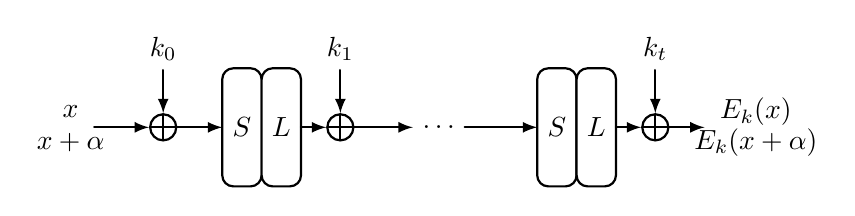
\begin{tikzpicture}[line cap=round]
            \tikzset{tikzxor/.style={draw,thick,circle,append after command={%
                    [shorten >=\pgflinewidth, shorten <=\pgflinewidth,]
                    (\tikzlastnode.north) edge[thick] (\tikzlastnode.south)
                    (\tikzlastnode.east) edge[thick] (\tikzlastnode.west)
                    }
                }
            }

            \node[tikzxor] (v1) at (-1.75,-4.25) {};
            \node[tikzxor] (v2) at (0.5,-4.25) {};
            \node[tikzxor] (v3) at (4.5,-4.25) {};

            \draw[thick, rounded corners, fill=white] (-1,-3.5) rectangle (-0.5,-5);
            \draw[thick, rounded corners, fill=white]  (-0.5,-3.5) rectangle (0,-5);
            \node at (-0.75,-4.25) {$S$};
            \node at (-0.25,-4.25) {$L$};

            \node (dots) at (1.75,-4.25) {$\dots$};
            \draw[thick, rounded corners, fill=white] (3,-3.5) rectangle (3.5,-5);
            \draw[thick, rounded corners, fill=white] (3.5,-3.5) rectangle (4,-5);
            \node at (3.25,-4.25) {$S$};
            \node at (3.75,-4.25) {$L$};

            \node (k0) at (-1.75,-3.25) {$k_0$};
            \draw [thick,-latex](k0) -- (v1);

            \node (k1) at (0.5,-3.25) {$k_1$};
            \draw [thick,-latex](k1) -- (v2);

            \node (kt) at (4.5,-3.25) {$k_t$};
            \draw [thick,-latex](kt) -- (v3);

            \node (x) at (-2.75,-4.25) {};
            \node [xshift=-5pt,yshift=2pt] at (x.north) {$x$};
            \node [xshift=-5pt,yshift=-2pt] at (x.south) {$x+\alpha$};
            \draw [thick,-latex](x) -- (v1);

            \node (Ekx) at (5.25,-4.25) {};
            \node [xshift=15pt,yshift=2pt] at (Ekx.north) {$E_k(x)$};
            \node [xshift=15pt,yshift=-2pt] at (Ekx.south) {$E_k(x+\alpha)$};
            \draw [thick,-latex](v3) -- (Ekx);

            \draw [thick,-latex](v1) -- (-1,-4.25);
            \draw [thick,-latex](0,-4.25) -- (v2);
            \draw [thick,-latex](v2) -- (dots);
            \draw [thick,-latex](dots) -- (3,-4.25);
            \draw [thick,-latex](4,-4.25) -- (v3);
        \end{tikzpicture}
%        \vspace{0.5em}
    \end{block}
    \end{minipage}

    \vspace{-0.5em}

    \begin{columns}[t,onlytextwidth]
        \begin{column}{0.3325\textwidth}
            \begin{block}{Easy parts}
            \vspace{-2pt}
                \begin{itemize}
                    \item Given a starting subspace, computing the trail is easy.
                    \item The effect of the linear layer $L$ to a subspace $U$ is clear:
                          \begin{equation*}
                              U \through{L} L(U)
                          \end{equation*}
                \end{itemize}
            \end{block}
        \end{column}

        \begin{column}{0.6\textwidth}
            \begin{block}{S-box: First Observation\vphantom{p}}
                \vspace{0.25em}
                For an S-box $S$ and $U \through{S} V$, because of the above lemma, $\forall x \in \F_2^n$ and $\forall u \in U$:
                \begin{align*}
                                                                &S(x) + S(x + u) \in V \\
                    \visible<2->{\Leftrightarrow \langle\alpha, &S(x) + S(x + u)\rangle = 0 \quad \forall \alpha \in V^\perp.}
                \end{align*}
                \visible<2->{%
                    By definition, $V^\perp$ is thus the set of zero-linear structures of $S$.\\[1em]
                }
            \end{block}
        \end{column}
    \end{columns}
\end{frame}

\begin{frame}{Possibility I}{The short one}
    \begin{columns}[t,onlytextwidth]
        \begin{column}{0.575\textwidth}
            \begin{block}{Theorem\vphantom{y}}
                Let $F : \F_2^{kn} \to \F_2^{kn}$ be an S-box layer that applies $k$ S-boxes with no non-trivial linear structures in parallel.
                Then every essential subspace trail $U \through{F} V$ is of the form
                \begin{equation*}
                    U = V = U_1 \times \cdots \times U_k,
                \end{equation*}
                where $U_i \in \set{\set{0}, \F_2^n}$.
            \end{block}
            \begin{center}
                In particular, in this case, bounds from activating S-boxes are optimal.
            \end{center}
        \end{column}
        \begin{column}{0.35\textwidth}
            \begin{block}{SPN Round: S-box layer}
                \vspace{0.5em}
                \centering
                \begin{tikzpicture}
                \foreach \z in {0,1,2,3} {%
                    \node[] (i\z) at ($(-0.25, \z*3em)+(0,0.35)$) {};
                    \node[] (o\z) at ($(0, \z*3em)+(3em,0.35)$) {};
                    \draw[thick,solid] (i\z) -- (o\z.center);
                }

                %% SBoxes
                \foreach \z in {0,1,2,3} {%
                    \node[draw,thick,solid,minimum width=2em,minimum height=2.75em,fill=white] (sl\z) at ($(i\z) + (2em,0em)$) {$S$};
                }

                \draw[draw=none] (i1) -- node[left,xshift=-1em] (U) {$U = $} (i2);
                \draw[draw=none] (i0) -- node[left] (x1) {$\times$} (i1);
                \draw[draw=none] (i1) -- node[left] (x2) {$\times$} (i2);
                \draw[draw=none] (i2) -- node[left] (x3) {$\times$} (i3);
                \node at (i0) [xshift=-6pt] (U0) {$U_0$};
                \node at (i1) [xshift=-6pt] (U1) {$U_1$};
                \node at (i2) [xshift=-6pt] (U2) {$U_2$};
                \node at (i3) [xshift=-6pt] (U3) {$U_3$};

                \draw[draw=none] (o1) -- node[left,xshift=37pt] (V) {$ = V$} (o2);
                \draw[draw=none] (o0) -- node[left,xshift=17pt] (y1) {$\times$} (o1);
                \draw[draw=none] (o1) -- node[left,xshift=17pt] (y2) {$\times$} (o2);
                \draw[draw=none] (o2) -- node[left,xshift=17pt] (y3) {$\times$} (o3);
                \node at (o0) [xshift=10pt] (V0) {$V_0$};
                \node at (o1) [xshift=10pt] (V1) {$V_1$};
                \node at (o2) [xshift=10pt] (V2) {$V_2$};
                \node at (o3) [xshift=10pt] (V3) {$V_3$};
                \end{tikzpicture}
                \vspace{0.5em}
            \end{block}
        \end{column}
    \end{columns}
\end{frame}

\begin{frame}{Possibility I}{Algorithm}
    \begin{columns}[t,onlytextwidth]
        \begin{column}{0.5\textwidth}
            \begin{block}{Algorithm}
                \begin{minipage}[t][30pt][t]{\textwidth}
                \begin{itemize}
                    \item Simply (de-)activate S-boxes
                    \item Compute resulting subspace trail
                \end{itemize}
                \end{minipage}
            \end{block}
        \end{column}
        \begin{column}{0.4\textwidth}
            \begin{block}{Complexity (No.\ of starting $U$s)}
                \begin{minipage}[t][30pt][t]{\textwidth}
                \vspace*{0pt}
                For $k$ S-boxes: $2^k$ (can be further decreased to $k$).
                \end{minipage}
            \end{block}
        \end{column}
    \end{columns}
    \vspace{0.5em}
    This approach is independent of the S-box, \ie/ any S-box without linear structures behaves the same with respect to subspace trails.
    \visible<2->{%
    \begin{minipage}{0.9775\textwidth}
    \begin{block}{The problem with S-boxes that have linear structures}
        Subspace trails through S-box layers with \emph{one}-linear structures are not necessarily a direct product of subspaces (see \eg/ Present).
    \end{block}
    \end{minipage}
    }
\end{frame}

\begin{frame}{Possibility II}{The long one, but only the idea}
    \begin{columns}[t,onlytextwidth]
        \begin{column}{0.55\textwidth}
            \begin{block}{Observation\vphantom{g}}
                \vspace{0.25em}
                If $U_1 \through{F} U_2$ is a subspace, then for any $V_1 \subseteq U_1$ there exists a $V_2 \subseteq U_2$, \st/ $V_1 \through{F} V_2$:
                \begin{equation*}
                \begin{aligned}
                    & U_1 & \stackrel{F}{\longrightarrow}\ &\ U_2 \\
                    & \rotatebox[origin=c]{90}{$\subseteq$} & &\ \rotatebox[origin=c]{90}{$\subseteq$} \\
                    & V_1 & \stackrel{F}{\longrightarrow}\ &\ V_2
                \end{aligned}
                \end{equation*}
            \end{block}
            \visible<2->{%
            \begin{block}{Complexity (Size of $\mathbb{W}$)}
                For an S-box layer $F : \F_2^{kn} \to \F_2^{kn}$ with $k$ S-boxes, each $n$-bit: $\abs{\mathbb{W}} = k \cdot (2^n-1)$
            \end{block}
            }
        \end{column}
        \begin{column}{0.4\textwidth}
            \visible<2->{%
            \begin{block}{Algorithm Idea}
                \begin{minipage}[t][146.5pt][t]{\textwidth}
                \vspace{1em}
                \begin{itemize}
                    \item Find a good set $\mathbb{W}$, \st/ for any possible subspace trail over the S-box layer $U \through{F} V$, there is an element $W \in \mathbb{W}$ \st/ $\set{W} \subseteq V$.
                \vspace{1em}
                    \item Compute the subspace trails for any starting point $W \in \mathbb{W}$.
                \end{itemize}
                \vspace{1em}
                \end{minipage}
            \end{block}
            }
        \end{column}
    \end{columns}
\end{frame}

%\begin{frame}{Results}{No linear structures}
%    \begin{block}{SPN ciphers with S-boxes without linear structures}
%        \centering
%        \renewcommand{\arraystretch}{1.2}
%        \begin{tabular}{lrrrr}
%            \toprule
%            Cipher                            & $r_e$ & $d$ & $r_d$ & $d$ \\
%            \midrule
%            AES                               &  2  &  32 &     2    &  32 \\ \rowcolor{gray!10}
%            Anubis                            &  2  & 104 &    ---   & --- \\
%            Klein                             &  3  &  60 &     2    &  32 \\ \rowcolor{gray!10}
%            Kuznyechik                        &  1  &   8 &     1    &   8 \\
%            Prince                            &  2  &  16 &     2    &  16 \\ \rowcolor{gray!10}
%            Qarma                             &  2  &  36 &     2    &  36 \\
%            \bottomrule
%        \end{tabular}
%    \end{block}
%\end{frame}
%
%\begin{frame}{Results}{One-linear structures}
%    \begin{block}{SPN ciphers with S-boxes with linear structures}
%        \centering
%        \renewcommand{\arraystretch}{1.2}
%        \begin{tabular}{lrrrrcrrrr}
%            \toprule
%                        & \multicolumn{4}{c}{LS} & & \multicolumn{4}{c}{\visible<2->{No LS}} \\
%            Cipher      & $r_e$   &   $d$   &    $r_d$   &  $d$  & & \visible<2->{$r_e$} & \visible<2->{$d$} & \visible<2->{$r_d$} & \visible<2->{$d$} \\
%            \midrule
%            Ascon       &   3     &   298   &      1     &  125  & & \visible<2->{3} & \visible<2->{ 310} & \visible<2->{1} & \visible<2->{155} \\ \rowcolor{gray!10}
%            Gift        &   3     &    60   &      3     &   60  & & \visible<2->{2} & \visible<2->{  16} & \visible<2->{2} & \visible<2->{ 16} \\
%            Keccak      &   2     &   546   &      1     &  169  & & \visible<2->{2} & \visible<2->{1290} & \visible<2->{1} & \visible<2->{270} \\ \rowcolor{gray!10}
%            Present     &   3     &    43   &      3     &   63  & & \visible<2->{2} & \visible<2->{  16} & \visible<2->{2} & \visible<2->{ 16} \\
%            Pride       &   2     &    31   &      2     &   34  & & \visible<2->{2} & \visible<2->{  56} & \visible<2->{1} & \visible<2->{ 40} \\ \rowcolor{gray!10}
%            Qarma       &   2     &    36   &      2     &   36  & & \visible<2->{2} & \visible<2->{  36} & \visible<2->{2} & \visible<2->{ 36} \\
%            Serpent     &   2     &    88   &      2     &   62  & & \visible<2->{2} & \visible<2->{ 100} & \visible<2->{2} & \visible<2->{ 68} \\ \rowcolor{gray!10}
%            Skinny64    &   5     &    48   &      5     &   48  & & \visible<2->{4} & \visible<2->{  48} & \visible<2->{4} & \visible<2->{ 48} \\
%            Skinny128   &   5     &    96   &      5     &   96  & & \visible<2->{5} & \visible<2->{  96} & \visible<2->{5} & \visible<2->{ 96} \\ %\rowcolor{gray!10}
%            \bottomrule
%        \end{tabular}
%    \end{block}
%\end{frame}

\begin{frame}{Conclusion/Questions}{Thank you for your attention!}
    \begin{columns}
        \begin{column}{0.5\textwidth}
            \begin{block}{Main Result}
                \begin{itemize}
                    \item Provable bound length of \emph{every possible} subspace trail in SPN cipher
                \end{itemize}
            \end{block}
            \begin{block}{Open Problems}
                \begin{itemize}
                    \item Other structures then SPNs?
                    \item Truncated Differentials?
                \end{itemize}
            \end{block}
        \end{column}
        \begin{column}{0.39\textwidth}
        \begin{figure}[!htb]
            
\includegraphics[height=50mm]{data/flickr/questionmark.png}
        \end{figure}
        \end{column}
    \end{columns}
    \blfootnote{\scriptsize Mainboard \& Questionmark Images: flickr}
\end{frame}

\begin{frame}[allowframebreaks]{References}
    \tiny
    \printbibliography{}
\end{frame}
